\documentclass[addpoints]{exam}

\usepackage{caption}
\usepackage{graphbox}
\usepackage{hyperref}
\usepackage{multirow}
\usepackage{pythonhighlight}
\usepackage{ragged2e}
\usepackage{subcaption}
\usepackage{tabularx}
\usepackage{titling}
\usepackage{xcolor}
\usepackage{float}

% Header and footer.
\pagestyle{headandfoot}
\runningheadrule
\runningfootrule
\runningheader{CS 201, Spring 2023}{HW 3: Hash Tables and AVL Trees}{\theauthor}
\runningfooter{}{Page \thepage\ of \numpages}{}
\firstpageheader{}{}{}

\qformat{{\large\bf \thequestion. \thequestiontitle}\hfill[\totalpoints\ points]}
% \qformat{{\large\bf \thequestion. \thequestiontitle}\hfill}
\boxedpoints

\printanswers

\graphicspath{{images/}}

\newcommand\colheader[1]{\multicolumn{1}{c}{#1}} % Note: no vertical bars

\title{Homework 3: Hash Tables and AVL Trees}
\author{unknown}  % <=== Enter your team name.
\date{Habib University\\Spring 2023}

\begin{document}
\maketitle
\part{Game of Life}
\label{sec:imgops}

\begin{quotation}
  \href{https://en.wikipedia.org/wiki/Conway's_Game_of_Life}{Conway’s Game of Life} is a simple simulation with surprisingly complex behavior. We start with a simple 2D grid of cells. Each cell can be either alive or dead. The rules are:
  \begin{itemize}
    \item A live cell stays alive if it has two or three live neighbors.
    \item A dead cell becomes alive if it has exactly three live neighbors.
  \end{itemize}
  We start with a certain set of cell states and then iterate, applying the rules to every cell at each iteration. Despite their simplicity, these rules can produce amazingly complicated behavior.
\end{quotation}
\raggedleft --- A flexible implementation of Conway's Game of Life \cite{gol_impl}
\justify
The rules above are slightly modified from their original formulation so as to be more amenable to our eventual implementation.

\section*{Initial Configurations}

The game begins with an initial configuration of live cells. This constitutes the starting state of the game. As the rules of the game are deterministic, the starting state completely determines all subsequent states of the game. Some initial configurations result in interesting behavior and have led to the identification of certain classes of patterns.
\begin{description}
  \item[Still Life] These patterns are not affected by further iterations of the game and stay unchanged as the game proceeds.
  \item[Oscillators] These patterns recur after a fixed number of iterations which are called the \textit{period} of the oscillator.
  \item[Spaceships] These are oscillators that change position or \textit{glide} across the grid.
\end{description}

\begin{figure}[!h]
  \centering
  \begin{tabular}{cc}
    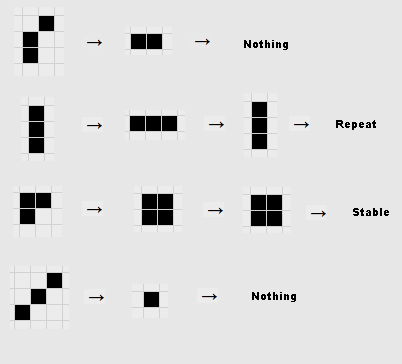
\includegraphics[width=.48\textwidth]{pattern1}
     & 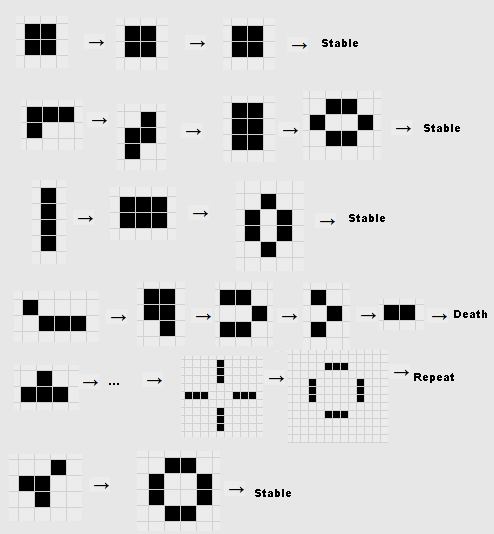
\includegraphics[width=.48\textwidth]{pattern2}
  \end{tabular}
  \caption{Evolution of the game from some initial states, taken from \cite{chaos}.}
\end{figure}


\section*{Computation}
\begin{quotation}
  It's possible even, to create patterns which emulate logic gates (and, not, or, etc.) and counters. Building up from these, it was proved that the Game of Life is Turing Complete \cite{wp_turing}, which means that with a suitable initial pattern, one can do any computation that can be done on any computer. Later, Paul Rendell actually constructed a simple Turing Machine as a proof of concept, which can be found here \cite{gol_turing}.
\end{quotation}
\raggedleft --- Chaos and Fractals: Conway's Game of Life \cite{chaos}
\justify

\section*{Visualization}

As the Game of Life is a dynamic system, i.e. its state changes with each iteration, it is best viewed as an animation which this document is unable to present. See Wikipedia \cite{wp_gol} or any of the other pages linked in this document for helpful animations. There are also many inspired and inspiring videos on YouTube including \cite{yt_gol}.

\section*{Implementation Details and Tasks}

An implementation of Conway's Game of Life is provided in the accompanying \texttt{src/} folder. The required functionality and components are defined in several files as follows.
\begin{description}
  \item[\texttt{game.py}] provides the \pyth{Game} class and also a \pyth{main()} function to run the game.
  \item[\texttt{life.py}] provides the \pyth{Life} and \pyth{Config} classes. \pyth{Life} encodes the state of the game and \pyth{Config} contains various configuration options. Both are used by the \pyth{Game} class.
  \item[\texttt{hashtables.py}] provides the abstract classes \pyth{MySet} and \pyth{MyDict} and contains declarations of the classes \pyth{ChainedSet}, \pyth{ChainedDict}, \pyth{LinearSet}, and \pyth{LinearDict} which derive from the abstract classes. You have to implement the derived classes so as to override and implement the interface defined in the abstract classes. These classes are required by the \pyth{Life} class in order to store and update the state of the game.
\end{description}

\section*{Class details}

\paragraph{\pyth{Life}} Every instance is initialized with a starting configuration which is stored using two different hash tables.
\begin{description}
  \item[\texttt{self.\_alive}] stores the two-dimensional $(x,y)$ coordinates of \texttt{live cells}.
  \item[\texttt{self.\_nbr\_count}] stores \textit{neighbor information} as key-value pairs where each key is an $(x,y)$ coordinate of a cell with \textit{live neighbors} and its value is the count of its live neighbors.
\end{description}

The hash tables store not only the initial configuration but, once the game starts, they store the state of the game at the end of each iteration. During each iteration, the live cells have to be used to populate neighbor information which in turn must be used to update the live cells for the next iteration. This is already coded in the \texttt{step} method of \texttt{Life}. \textit{Do not modify} the implementation of this class.

\paragraph{\pyth{Game}} It runs a \texttt{Life} instance according to the provided configurations with an option for animation. In the animation system used, the origin, $(0,0)$, is at the top left of the window. This class is provided for your testing. \textit{You may modify} it as per your needs.


All files are fully documented. Please refer to in-file documentation for further details.

\section*{Task}

Your task is to implement the \pyth{MySet} and \pyth{MyDict} subclass in \texttt{src/hashtables.py} using two different conflict resolution methods. Specifically, you have to implement the following classes which are utilized in the implementation of \texttt{Life}.
\begin{description}
  \item[\texttt{ChainedSet}] A hash table that implements the \pyth{MySet} interface using chaining for conflict resolution.
  \item[\texttt{ChainedDict}] A hash table that implements the \pyth{MyDict} interface as an associative container and uses chaining for conflict resolution.
  \item[\texttt{LinearSet}] A hash table that implements the \pyth{MySet} interface using linear probing for conflict resolution.
  \item[\texttt{LinearDict}] A hash table that implements the \pyth{MyDict} interface as an associative container and uses linear probing for conflict resolution.
\end{description}
The conflict resolution strategy to use is indicated through a parameter passed to \pyth{Life} at the time of initialization.

\section*{Requirements}

You will need to install the following modules.
\begin{description}
  \item [\texttt{typing}] to support certain type hints used in the code
  \item [\texttt{time}] to support animation of the game
\end{description}

\section*{Tips}

Below are some tips to gain a better understanding of the homework and facilitate your work for this assignment.
\begin{itemize}
  \item Go over the provided implementation in order to understand the role and function of each class and its methods.
  \item Run the game using native python types as described below.
  \item Run the game using different initial configurations defined in the \pyth{Config} class.
  \item Feel free to add other initial configurations defined to the \pyth{Config} class.
  \item Feel free to modify the configuration options in \pyth{main()} in order to observe their effect.
\end{itemize}

\section*{Testing}

You can test the framework by initializing \pyth{self._alive} and \pyth{self._nbr_count} with a native python \pyth{set} and \pyth{dict} instance respectively in \pyth{Life.__init__()}.

Once you have successfully implemented the hashtables, you can test your code by running the provided \texttt{pytest} files. These will also be used by GitHub to auto-grade your submission.

\section*{Credits}

The Game of Life segment is adapted from \cite{gol_impl}.

\newpage
\part{Scientific Publications}

You are working for a startup that provides a search engine for scientific publications. The search engine allows users to search for publications by 
entering keywords related to the topic they are interested in. Your job is to create an AVL Tree that will be used to index the publications and speed up the search process.

The startup has a large database of scientific publications, each containing multiple sentences. Your task is to create an AVL Tree 
where the key is a keyword and the value is a list of tuples where the first element is the index of the document in which the 
keyword is found and the second element is the index of the sentence in the document where the keyword is found.

The search engine will use the AVL Tree to quickly retrieve the list of publications that contain a given keyword. Your goal is to create an efficient implementation of the AVL Tree that can handle the large amount of data and provide fast search times.
In this programming assignment, you are given a data file \texttt{data/publications.csv} that contains records of publications. Each records contains the following attributes:
\begin{itemize}
  \item Title
  \item Abstract
\end{itemize}

\section*{Implementation Details and Tasks}
\begin{itemize}
  \item Implement the \pyth{AVLTree} class in the accompanying file, \pyth{avl_tree.py}, in the accompanying \texttt{src/} sub-folder.
  \item In the \pyth{AVLTree} class, implement the following methods:
  \begin{itemize}
    \item \pyth{insert (key: str,value: Tuple[int,int]) -> None}: Inserts a \texttt{(doc\_id, sen\_id)} tuple into the AVL Tree with the given keyword .
    \item \pyth{search (key: str) -> List[Tuple[int,int]]}: Searches for a keyword in the AVL Tree and returns a list of \texttt{(doc\_id, sen\_id)} corresponding to the keyword. 
    Returns an empty list if the keyword is not found.
    \item \pyth{rotate_left(node: AVLTreeNode) -> None}: Performs a left rotation on the subtree rooted at the given node.
    \item \pyth{rotate_left(node: AVLTreeNode) -> None}: Performs a right rotation on the subtree rooted at the given node.
    \end{itemize}
  \item The \pyth{Publication} class which loads the file, prepossesses the data and uses the \pyth{AVLTree} class has already been implemented in the accompanying file, \pyth{publication.py}, in the accompanying \texttt{src} subfolder.
\end{itemize}

\section*{Input and Output}
In the following examples, the table \ref{tab:inp} displays shows some sample documents based on which the AVL Tree is constructed. The program takes as input a keyword, searches the AVL Tree for the given keyword and then returns a list of tuples \texttt{(doc\_id,sen\_id)}
\begin{table}[h!]
  \centering
  \begin{tabular}{|c|c|}
    \hline
    Title & Abstract \\ \hline
    Doc1 & This is the first document. \\ \hline
    Doc2 & This is the second document.\\ \hline
    Doc3 & This is the third document. \\ \hline
  \end{tabular}
  \caption{Sample Documents}
  \label{tab:inp}
\end{table}
\newpage
\begin{table}[h!]
  \centering
  \begin{tabular}{|c|c|}
    \hline
    Input & Output \\ \hline
    document &  (0, 0), (1, 0), (2, 0) \\ \hline
    third & (2,0) \\ \hline
  \end{tabular}
  \caption{Sample Test Cases}
  \label{tab:test}
\end{table}

\section*{Requirements}

You will need to install the following modules.
\item [\texttt{nltk}]  to remove stop words, punctuation, and stem the words.



\section*{Testing}
Once you have successfully implemented the methods, you can test your code by reading from the accompanying data file, \texttt{data/publications.csv}, and performing queries on it. For grading purposes, your submission will
be tested automatically by GitHub using the accompanying \texttt{pytest} file, \texttt{test\_avl}.py.


\newpage
\begin{thebibliography}{9}

  \bibitem{wp_gol}
  Conway’s Game of Life, \url{https://en.wikipedia.org/wiki/Conway%27s_Game_of_Life}, last accessed on 16 Feb 2022.

  \bibitem{chaos}
  Chaos and Fractals: Conway’s Game of Life, \url{http://pi.math.cornell.edu/~lipa/mec/lesson6.html}, last accessed on 16 Feb 2022.

  \bibitem{gol_impl}
  A flexible implementation of Conway's Game of Life, \url{https://www.refsmmat.com/posts/2016-01-25-conway-game-of-life.html}, last accessed on 16 Feb 2022.

  \bibitem{wp_turing}
  Turing complete, \url{https://simple.wikipedia.org/wiki/Turing_complete}, last accessed on 16 Feb 2022.

  \bibitem{gol_turing}
  This is a Turing Machine implemented in Conway's Game of Life., \url{http://www.rendell-attic.org/gol/tm.htm}, last accessed on 16 Feb 2022.

  \bibitem{yt_gol}
  epic conway's game of life, \url{https://www.youtube.com/watch?v=C2vgICfQawE}, last accessed on 16 Feb 2022.
\end{thebibliography}

\end{document}
%%% Local Variables:
%%% mode: latex
%%% TeX-master: t
%%% End:
